
%----------------------------------------------------------------------------------------
% 	Template: Abschlussarbeiten des Studiengangs Angewandte Informatik an der HTW Berlin
% 	C. Schmidt 
%----------------------------------------------------------------------------------------
%	Pakete und Konfigurationen
%----------------------------------------------------------------------------------------
%\documentclass[twoside,twocolumn]{article}
%\documentclass[german,a4paper,12pt,oneside]{scrbook}
\documentclass[oneside,bibliography=totocnumbered,BCOR=5mm]{scrbook}% Voreinstellungen entfernt.

\usepackage[latin1]{inputenc}
\usepackage{amsmath, amsthm, amssymb}
\usepackage[ngerman,english]{babel} % Language hyphenation and typographical rules
\usepackage{marvosym}
\usepackage{graphics}
\usepackage{csquotes}
\usepackage{acronym} % List of Abbreviations generator
\newtheorem{satz}{Satz}[chapter]
\theoremstyle{definition} 
\newtheorem{definition}[satz]{Definition} 
\theoremstyle{definition} 
\newtheorem{lemma}[satz]{Lemma} 
\theoremstyle{definition} 
\newtheorem{bemerkung}[satz]{Bemerkung}
\theoremstyle{definition} 
\newtheorem{korollar}[satz]{Korollar} 
\theoremstyle{definition}
\newtheorem{beispiel}[satz]{Beispiel} 
\theoremstyle{definition} 
\newtheorem{algorithmus}{Algorithmus} 
\newenvironment{beweis}{\begin{proof}[Beweis]}{\end{proof}}
\usepackage[hyphens]{url}
\usepackage{hyperref}



%----------------------------------------------------------------------------------------
%	BIB.-Datei und Quellenverwaltung
%----------------------------------------------------------------------------------------
\usepackage[backend=bibtex,style=numeric]{biblatex}
\addbibresource{thesis.bib}
%\usepackage{natbib} % use natbib for references 
%----------------------------------------------------------------------------------------

\usepackage[sc]{mathpazo} % Use the Palatino font
\usepackage[T1]{fontenc} % Use 8-bit encoding that has 256 glyphs
\linespread{1.05} % Line spacing - Palatino needs more space between lines
\usepackage{microtype} % Slightly tweak font spacing for aesthetics

\usepackage[hmarginratio=1:1,top=32mm,columnsep=20pt]{geometry} % Document margins
\usepackage[hang,small,labelfont=bf,up,textfont=it,up]{caption} % Custom captions under/above floats in tables or figures
\usepackage{booktabs} % Horizontal rules in tables
\usepackage{lettrine} % The lettrine is the first enlarged letter at the beginning of the text
\usepackage{enumitem} % Customized lists
\setlist[itemize]{noitemsep} % Make itemize lists more compact

% \usepackage{abstract} % Allows abstract customization
% \renewcommand{\abstractnamefont}{\normalfont\bfseries} % Set the "Abstract" text to bold
% \renewcommand{\abstracttextfont}{\normalfont\small\itshape} % Set the abstract itself to small italic text

\usepackage{titlesec} % Allows customization of titles
% \renewcommand\thesection{\Roman{section}} % Roman numerals for the sections
% \renewcommand\thesubsection{\roman{subsection}} % roman numerals for subsections
\titleformat{\section}{\Large\bfseries\sffamily}{\thesection.}{1em}{} % Change the look of the section titles
\titleformat{\subsection}{\large\bfseries\sffamily}{\thesubsection.}{1em}{} % Change the look of the section titles

\usepackage{fancyhdr} % Headers and footers
\pagestyle{fancy} % All pages have headers and footers
\fancyhf{} % Blank out the default header and the default footer
\fancyhead[L]{\rightmark} % Custom header text
\fancyhead[C]{} % Custom header text
\fancyfoot[RO,LE]{\thepage} % Custom footer text

\usepackage{titling} % Customizing the title section



%----------------------------------------------------------------------------------------
%	Listings
%----------------------------------------------------------------------------------------

\usepackage{listings}
\usepackage{color}

\definecolor{mygreen}{rgb}{0,0.6,0}
\definecolor{mygray}{rgb}{0.5,0.5,0.5}
\definecolor{mymauve}{rgb}{0.58,0,0.82}

\lstset{ 
  backgroundcolor=\color{white},   % choose the background color; you must add \usepackage{color} or \usepackage{xcolor}; should come as last argument
  basicstyle=\footnotesize,        % the size of the fonts that are used for the code
  breakatwhitespace=false,         % sets if automatic breaks should only happen at whitespace
  breaklines=true,                 % sets automatic line breaking
  captionpos=b,                    % sets the caption-position to bottom
  commentstyle=\color{mygreen},    % comment style
  deletekeywords={...},            % if you want to delete keywords from the given language
  escapeinside={\%*}{*)},          % if you want to add LaTeX within your code
  extendedchars=true,              % lets you use non-ASCII characters; for 8-bits encodings only, does not work with UTF-8
  firstnumber=1,                   % start line enumeration with line 1000
  frame=single,	                   % adds a frame around the code
  keepspaces=true,                 % keeps spaces in text, useful for keeping indentation of code (possibly needs columns=flexible)
  keywordstyle=\color{blue},       % keyword style
  language=Octave,                 % the language of the code
  morekeywords={*,...},            % if you want to add more keywords to the set
  numbers=left,                    % where to put the line-numbers; possible values are (none, left, right)
  numbersep=5pt,                   % how far the line-numbers are from the code
  numberstyle=\tiny\color{mygray}, % the style that is used for the line-numbers
  rulecolor=\color{black},         % if not set, the frame-color may be changed on line-breaks within not-black text (e.g. comments (green here))
  showspaces=false,                % show spaces everywhere adding particular underscores; it overrides 'showstringspaces'
  showstringspaces=false,          % underline spaces within strings only
  showtabs=false,                  % show tabs within strings adding particular underscores
  stepnumber=1,                    % the step between two line-numbers. If it's 1, each line will be numbered
  stringstyle=\color{mymauve},     % string literal style
  tabsize=2,	                     % sets default tabsize to 2 spaces
  title=\lstname                   % show the filename of files included with \lstinputlisting; also try caption instead of title
}



%----------------------------------------------------------------------------------------
%	Haupttextteil
%----------------------------------------------------------------------------------------

\begin{document}

% Titelseite
% \pagestyle{empty}       % keine Seitennummer
\begin{titlepage}
\begin{center}

\includegraphics{assets/HTW_Berlin_Logo_farbig.jpg}
\linebreak[4]
\linebreak[4]
\linebreak[4]
\linebreak[4]
\textit{\large Development of a Chrome Extension for Personalized Filter Suggestions}
\linebreak[4]
\linebreak[4]
\linebreak[4]
Abschlussarbeit 
\linebreak[4]
\linebreak[4]
zur Erlangung des akademischen Grades: 
\linebreak[4]
\linebreak[4]
\textbf{Bachelor of Science (B.Sc.)}
\linebreak[4]
\linebreak[4]
an der
\linebreak[4]
\linebreak[4]
Hochschule f\"ur Technik und Wirtschaft (HTW) Berlin
\linebreak[4]
Fachbereich 4: Informatik, Kommunikation und Wirtschaft
\linebreak[4]
Studiengang \textit{Angewandte Informatik}
\linebreak[4]
\linebreak[4]
\linebreak[4]
1. Gutachter\_in: Prof. Dr. Elena Sch\"uler\linebreak[4]
2. Gutachter\_in: Birol Aksu\linebreak[4]
\linebreak[4]
\linebreak[4]
\linebreak[4]
\linebreak[4]
Eingereicht von Sunan Regi Maunakea 566144
\linebreak[4]
\linebreak[4]
\linebreak[4]
\linebreak[4]
22. August 2022

\end{center}
\end{titlepage}
\newpage

\thispagestyle{empty}       % keine Seitennummer
% vertikaler Leerraum
\vspace*{2.2cm}
\noindent %kein Einzug
{\Huge Danksagung}\\
\vspace*{1.6cm} \\

% Kopfzeilen (automatisch erzeugt)
\pagestyle{headings}
[Text der Danksagung]

% Seite mit Abstracts
\newpage
\thispagestyle{empty}       % keine Seitennummer
\section*{Zusammenfassung}
[Text der Zusammenfassung]

\section*{Abstract}
[Summary of the thesis]

\clearpage

\pagenumbering{roman}

\tableofcontents
\listoffigures

\newpage
\pagenumbering{arabic}

\newpage
\chapter{Introduction}
The way we access digital information directly has fundamentally altered how information is retrieved, allowing us to create search engines that can significantly speed up the search process by allowing users to jump straight to the content they are interested in without having to navigate through convoluted systems. This instant gratification far outperforms previous methods of flipping through physical pages. But as digital information access has grown, so has the amount of information that is available on any given subject. As a result, finding the desired product would be difficult even with instant access via search.

The idea that the more options available, the better, and that human desire for choice is limitless are both prevalent in modern society. One study showed that the existence of choice increases motivation and enhances performance on doing tasks \autocite{zuckerman1978importance}. However, another study has shown that although having more choices might appear desirable, it may sometimes have negative effects on human motivation \autocite{iyengar2000choice}. To resolve this issue, filters are introduced. Filters help users find informations faster. Rich information systems have recently begun to provide faceted navigation, which basically extends the idea of filters into a complex structure that attempts to describe all the different aspects of an object in order to maximize flexibility in retrieving information \autocite{whitenton2014filters}. Nevertheless, using this more flexible and more useful tool requires multiple steps, especially if users repeatedly search for the same information.

\section{Objectives}
The goal of this thesis is to design and implement a filtering suggestions tool, consisting of a client component, to circumvent the numerous steps involved in searching for an article or a product on a website. Thereby, a clear presentation and its development will be discussed as well as the technical background of the extension. The client component is implemented as a Google Chrome extension. To achieve a user-friendly extension, it is critical to provide the user with access to useful and clear information, so the extension to be developed will be compactly customized to one view, allowing the user to see their frequently visited websites.

\section{Structure of the Thesis}
The thesis is divided into four chapters. First, the descriptions of filtering, exploratory search and faceted search are provided. In addition, the anatomy of a URL as well as search and filtering usage in a URL are defined. Finally, the fundamentals of the technologies used are then explained in chapter 2. Further on, in chapter 3 the experimental methodology used for studies conducted with the Chrome extension is described. The extension's implementation and use in a practical situation are discussed in some detail in chapter 4 along with some lessons learned. Subsequently, the extension is evaluated and analyzed. Finally, problems are identified and an outlook for possible improvements of the extension is given.

\newpage
\chapter{Theoretical Basis}
In the first section, this chapter describes the concept of URL and how resources are searched and filtered using URL parameters. The second section describes the concept of a browser extension. Furthermore, the choice of implementation browser is defined with which it is possible to develop an extension. The third chapter covers the architecture of a Chrome Extension. Finally, the framework for the extension's UI implementation is elucidated.

% TODO: add the theory behind the problem that we want to solve by
% creating the extension, which is, what is the problem of having
% too many options?

% Uniform Resource Locator
\section{Uniform Resource Locator}
Uniform Resource Locator, or URL, is a compact string representation for a resource available via the Internet \autocite{berners1994uniform}. URLs are used to "locate" resources, by providing an abstract identification of the resource location. These resources could be an image, a CSS file, an HTML page, etc. In practice, there are a few exceptions, the most frequent of which is a URL leading to a resource that has either relocated or vanished. After locating a resource, a system may carry out a number of actions on it, which can be described by phrases like "access", "update", "replace", and "find attributes". For each URL scheme, only the "access" method needs to be supplied. Here is an example of an HTTP URL: \texttt{http://www.example.com/software/index.html}

\subsection{Anatomy of a URL}
A URL is made up of various components, some of which are required and others which are not \autocite{mozilla2022url}. The most important parts are provided in the following sections:

\subsection*{Scheme}
The scheme, which indicates the protocol that the browser must use to request the resource, is the first part of the URL. A protocol is a set method for exchanging or transferring data around a computer network. The most common protocol is HTTP which stands for Hypertext Transfer Protocol. Nowadays most websites use HTTPS protocol which stands for Hypertext Transfer Protocol Secure.

\subsection*{Authority}
The authority is then separated from the scheme by the character pattern \texttt{://}. If the authority is present, it includes both the host (e.g., \texttt{www.example.com}) and the port (80), separated by a colon:

\begin{itemize}
  \item The host name identifies the host that holds the resource. A server provides services in the name of the host, but hosts and servers do not have a one-to-one mapping.
  \item The port number denotes the technical "gateway" used to access the web server's resources. It is typically omitted if the web server grants access to its resources via the HTTP protocol's standard ports. Otherwise, it is required.
\end{itemize}

\subsection*{Path}
The path identifies the specific resource in the host that the web client wants to access. For example, \texttt{/software/htp/cics/index.html}.

\subsection*{Query String}
A query is commonly found in the URL of dynamic pages. and is represented by a question mark followed by one or more parameters. The query directly follows the host name, path or port number. For example, this URL was generated by Google when doing a search for the word "query":

\begin{center}
  \url{https://www.google.com/search?q=query&rlz=1C5GCEM_enDE993DE993&oq=query&aqs=chrome..69i57j0i512l4j69i60l3.938j0j7&sourceid=chrome&ie=UTF-8}
\end{center}

\noindent This is the query part:

\begin{center}
  \url{?q=query&rlz=1C5GCEM_enDE993DE993&oq=query&aqs=chrome..69i57j0i512l4j69i60l3.938j0j7&sourceid=chrome&ie=UTF-8}
\end{center}

\subsection*{Anchor}
An anchor is a type of "bookmark" within the resource that instructs the browser to display the content located at that "bookmarked" location. For example, in an HTML document, the browser will scroll to the point where the anchor is defined; in a video or audio document, the browser will attempt to navigate to the time the anchor represents. It is important to note that the part following the \texttt{\#}, also known as the fragment identifier, is never sent to the server with the request.

\subsection{Search and Filter URL Parameters}
Search and filter URL parameters are parameters or query strings that add information to a specific URL. A search or filter parameter facilitates the search for a specific phrase or keyword within search engine results. They include what is requested while excluding irrelevant content. Aside from the functions mentioned above, the most common use cases for parameters are tracking, pagination, site search, sorting and filtering.

%Site Search
\section{Site Search}
Providing a search function that searches your Web pages is a design strategy that offers users a way to find content \autocite{w3c2016search}. Users can find content by searching for specific words or phrases without having to understand or navigate the site's structure. This can be a faster or easier way to find content on large sites. A great site search function is specific to the website and not only constantly indexes the site to ensure the most recent content is easily accessible, but it also guides users as they explore a website's content, assisting them in discovering content they may not have known they were interested in. The best site search products delight users by allowing them to quickly connect with the content they require while also collecting valuable data about the content and products that visitors are most interested in.


%Filters
\section{Filters}
The process of narrowing down a search based on predefined categories is known as filtering. These categories are frequently broad and based on a single dimension of the product. This allows user to quickly narrow down a large number of products to a more manageable set for further investigation.

Filters are broad categories defined by the business that do not change between searches, and they are frequently used behind the scenes. For example, an online clothing store might use "clothing type" as a filter, with four possible categories: shirts, pants, shoes, and accessories. When a website visitor clicks on "shirts" in the top navigation, the clothing type filter is applied, and the visitor sees only shirts on the results page.


%Facets and faceted search
\section{Facets and faceted search}
Facets, also known as facet filters, enable users to filter results by selecting values along different dimensions or facets \autocite{qu2021study}. It is widely used in e-commerce search engines and digital libraries where documents have rich metadata. Faceted search is a more granular method of finding products and results in a specific, targeted way that broad, one-size-fits-all filters do not allow.

Facets and faceted search are features of a well-designed user interface. Contextual facets that change depending on the item or category drive a user-friendly experience by guiding the user down the quickest path to the best result.


%Browser Extension
\section{Browser Extension}
Browser extensions or addons are third party programs, that can extend the functionality of browsers and improve users' browsing experience \autocite{some2019empoweb}. A browser extension, as opposed to a standard web page, is created specifically for a given browser and uses that browser's extension API. It was necessary to choose a browser as a result. There are frameworks that try to make it feasible to create an extension for several different browsers at once. Although the caliber of these frameworks was unclear, it was decided that the expense of potential problems and additional time spent debugging in many browsers outweighed the benefits.


%Chrome Extension Architecture
\section{Chrome Extension Architecture}
Extensions are built on web technologies such as HTML, JavaScript, and CSS. They run in a separate, sandboxed execution environment and interact with the Chrome browser \autocite{google2021what}. They also have access to the APIs that browsers provide for tasks like XMLHttpRequests and HTML5 features on web sites. The following files can be found in an extension:

\begin{itemize}
  \item A manifest.json file
  \item One or more HTML files
  \item Any other files such as CSS or JavaScript needed by the extension to run
\end{itemize}

The majority of extensions have a background page that contains their primary logic and state. They frequently also contain content scripts that can communicate with websites. Asynchronous message passing is used to communicate between the background page and the content scripts. Additionally, extensions can save data via localStorage and other HTML5 storage APIs.

\subsection*{Manifest Files}
A manifest.json file is required for each extension. It includes crucial information about the extension, such its name, version, scripts used for its content, minimum Chrome version, and permissions. The content-scripts field was the most crucial one for this expansion. Each study and content-related webpage need its own content script. Each one was defined in the scripts column, which also mapped each one to the appropriate URLs.

\subsection*{Content Scripts}
Content scripts are JavaScript files that are used on websites to add new functionality. They have full control to modify the entire web page because they can directly access the DOM of these web sites. The content script is injected into a tab when the web page is loaded, and runs in the same process space of the renderer of the web tab and can thus access its DOM objects. Injected content scripts in a tab can only communicate with the extension core via Chrome's IPC \autocite{liu2012chrome}.

\subsection*{Service Worker}
The Chrome extension platform switches from background pages to service workers in Manifest V3. A service worker is a script that your browser runs in the background, distinct from a web page, opening the door to features that don't need a web page or user input \autocite{chrome2021service}. This technology allows native-like experiences over the open web, including push notifications, robust offline support, background synchronization, and "Add to Home Screen." Service providers drew some of their inspiration from the background pages in Chrome Extensions, but improvements were added for the web.

Service workers are specialized JavaScript assets that act as proxies between web browsers and web servers. They aim to improve reliability by providing offline access, as well as boost page performance \autocite{chrome2021service}. Websites are gradually improved by service workers through a lifetime akin to that of platform-specific programs.


%React
\section{React}
React is a product of Facebook's engineering team, which is a JavaScript framework for creating user interfaces \autocite{gackenheimer2015introducing}. Because of its simplicity and straightforward but efficient development process, React is quite well-liked in the developer communities. Interactive user interfaces are simpler to develop with React. It effectively updates by accurately drawing each state's view's constituent parts, and it updates the application's data \autocite{islam2017reactjs}. The core objective of React is to provide the best possible rendering performance. Its strength comes from the focus on individual components. Using reusable components, it is found to be easy development for developers to design rich UI's. React incorporates with View part from MVC model \autocite{maratkar2021re}. React implements One Way dataflow so that it gets easier than traditional data binding. React uses virtual DOM it offers not so complex programming with faster execution. It makes use of composition to create intricate user interfaces out of simple building blocks known as Components \autocite{david2020building}.

\subsection*{Component}
Each component has a render method, which can either return HTML or another React component, and returns a description of what to render. A combination of HTML and Javascript known as JSX is used to describe what should be rendered. A more detailed explanation of JSX is included in the JSX section. It is possible to specify a component as a class or a function. Props and state are crucial components when creating React applications.

\subsection*{States and props}
The state of a component allows it to "remember" things, and it can change in response to user interaction or other application-wide actions. The State is optional; components without a state are referred to as presentational components. Components with a state are referred to as stateful components.

Immutable data supplied into a component during development is known as props, or properties. Because a component can function and seem differently depending on the properties supplied into it, props enable React components to be flexible and reusable.

Using props, data moves down the component tree in React. Callback functions are supplied as props so that a child component can communicate with its parent. Callback methods and other data must be passed down numerous layers in large React apps due to the component tree's depth. Props-drilling is a technique that results in tightly connected components and a less maintainable program. This is one of the reasons why complex React apps require architectural patterns.

\subsection*{Class-based components}
A class-based Component is created by extending the React.Component class. The state of a class-based component is updated using the method setState() and read by using this.state within the class. Using the setState() method makes the component re-render which is not the case when mutating the state directly. Class-based components include life-cycle methods that can be used to create more complex behavior. It also requires a render method to return JSX elements.

\subsection*{Life-cycle methods}
Life-cycle methods are built-in functions that are called whenever a state or prop updates, a component renders, is destroyed, or both.

\subsection*{Function components}
A pure function that takes props as input and outputs a JSX element is referred to as a function component. React Hooks are used to give the function component the same access to state and life-cycle methods as class-based components. In compared to class-based components, using function components with hooks might make React applications smaller and more manageable. There are a couple reasons why function component is preverable \autocite{phan2020react}:

\begin{itemize}
  \item Faster development, easier to read and test, debug and reusable; because function components do not have state and life-cycle-hook. Function component is a straightforward JavaScript function.
  \item Performance will be improved since function components are smaller and compiles more quickly than class components.
  \item There is no need to consider how to divide the component into a container and a standard UI component when utilizing a function component.
\end{itemize}

\subsection*{React Hooks}
For more complex function components, React Hooks are utilized; they "hook onto" React capabilities. React hook names begin with the word "use," per tradition. By default, state is absent from function component; however, the useState React hook can be used to keep state for the duration of the component. All hooks, including the useState one, are repeatable inside a single component.

Function components do not come with built-in life-cycle methods, but they can be added using the useEffect hook. By default, the useEffect hook will run a function for each time the component is re-rendered, but it may be modified to just run for specific modifications.

The useContext hook, which will be described in the Context API section, is another React hook. In addition to built-in hooks, custom hooks can be made, allowing functionality to be reused throughout components.

\subsection*{Virtual DOM}
For all components in the application, React generates a new View based on immutable states and props; a change to either a state or a prop causes the View to be re-rendered. The Views are now predictable and testable as a result. The user experience is negatively impacted by the time-consuming process of re-rendering views by swapping out the DOM for a new version, which also causes scrolling position and input information to be lost. Using a Virtual DOM, React provides a solution for this \autocite{david2020building}.

By establishing a new Virtual DOM subtree when data in the application changes and comparing it to the previous one, the Virtual DOM re-renders Views that need to update in an affordable manner without disrupting other DOM nodes. React determines the minimal number of DOM alterations required to match the virtual DOM with the real DOM. Javascript is used to do DOM manipulations, which are then queued up and executed in batches to save time. React takes care of manipulating the DOM to get to the various states, while developers utilize JSX to define how components should render in various states.

\subsection*{Context API}
The Context API is a built-in tool that allows data to be shared between React components without the need for props-drilling. The createContext method in the React library is used to initialize a Context, which can be used by several components in the component tree. A Provider present on the Context instance is used to add data to the Context and make it accessible to children components. The data for the Context is specified in the Provider, a component that has a single property named value and accepts variables, functions, or objects as values. The Context data can be retrieved from any child component using a Consumer that is also available on the Context instance by enclosing children components inside the Provider component. The application uses a variety of contexts for various purposes rather than being restricted to a single instance.

Context API's callback function inheritance allows a child component to change the state of a parent component. Context is used, according to the official documentation, to exchange information that is regarded as global for the tree of React components, such as whether a user is logged in, the application's theme, or the language preferences. Because they depend on information provided by context from another component, using context may reduce the reusability of components. UseContext functions as the Consumer and grants access to the data for a functional component encased in a Context Provider.

\subsection*{JSX}
A React extension called JSX makes it simple for web designers to change the DOM using straightforward HTML-style code. Additionally, as all current web browsers are supported by React JS, JSX is interoperable with any browser platform.

Most people find it helpful as a visual aid when working with UI inside the JavaScript code. It also allows React to show more useful error and warning messages \autocite{react2020introducing}. The advantages of JSX include the fact that it makes writing templates for users who are familiar with HTML simpler and faster. Performance improves when code is compiled into JavaScript \autocite{phan2020react}.

\newpage
\chapter{Methodology}
The initial idea of the thesis is first defined in the following chapter. In the second section, we look at some of the comparable programs that are already on the market. The third section discusses the resulting design considerations necessary for implementing the extension. The fourth section covers the software's design in light of the requirements. The decision to implement the technologies is described in the final section.

\section{Design Concept}
This thesis' original idea is to add an additional feature to Marta's customer-facing platforms. Marta\footnote{\emph{Marta} homepage: \url{https://www.marta.de/}} is currently best described as a marketplace between families requiring 24-hour care and caregivers. 24-hour care can be defined as a period of time spent living in the same household as the individual requiring care. This means that the primary responsibilities of caregivers are basic care and household chores. In addition, they provide assistance to the care recipient's relatives so that they can participate in activities of their choosing. Marta competes with more traditional agencies, where it can take days or even weeks to find a family for a newly registered caregiver or the other way around.

To compete in this rapidly growing industry, Marta would need to improve their product as an expanding startup that has gained a large number of users in recent months. One way in which Marta can provide a superior experience for both caregivers and families is by accelerating the matching process. The caregiver and family inquiry forms are intended to collect as much relevant information as possible for use during the matching phase. The matches are then generated based on the information from the inquiry. To streamline the process, the family is then presented with a number of caregiver profiles that are a good fit for their needs. Filtering capabilities are provided to expedite the search process. This includes the caregiver's earliest start date, German proficiency, disease experience, etc.

To meet the requirements of its users, Marta must implement a continually enhanced, user-friendly filtering capability. An example of a user-friendly filter would be to provide quick filter suggestions that the user can click once to display the desired results, as opposed to allowing users to repeatedly select the same filter manually. To determine which filter suggestions are the most beneficial, it is necessary to identify frequently used filters.

Within this realm of thought, the question of how to enhance the existing filtering functionality for a better user experience arose. An early idea was to create quick filters within the application that would suggest to users which filters they used most frequently. For instance, if a family is seeking a caregiver with level three German language proficiency, the German filter would be activated. Each filter application will be recorded in a relational database. The three most frequently used filters will be displayed as quick filters for all users to activate with a single click. In addition, the user can combine these quick filters to further narrow the search results.

The first issue with this concept was that it collected and stored filter usage data from every user without providing specific information about who used the filter and when. Each family has distinct search criteria. Therefore, the first concept would not be as advantageous to users. Additionally, we must remember that this strategy will only benefit those who actively use the platform. The second concern was that if filter recommendations were personalized for each user, the amount of data maintained would quickly grow to be quite substantial. It would be an inefficient use of storage space, especially as the number of filters and users increases. Not only would we develop quick filters for a single page, but also multiple. And each would necessitate the same quantity of storage space.

The idea was then elaborated upon, and a decision was made. Instead of integrating these quick filters directly into the platform, it would be preferable to create an extension that allows for even more personalized filter suggestions. The aforementioned problems can be resolved by creating an extension. The information that will be saved is user-specific and is stored in the browser of the end user, so the filter suggestions are not affected by the actions of other users. Moreover, search and filter is a common web design technique. It would benefit not only Marta's platform, but also Lacoste, Nike, Adidas, and other e-commerce websites. Moving it to an extension would provide users with the option to install it. And because this is a distinct capability with a different software architecture than Marta's primary platform, a new repository or codebase is created to make it easier to differentiate and manage.

\section{Existing Software}
This section covers the currently available applications or extensions that are similar but do not completely solve the aforementioned problem. There exists a considerable amount of software for manipulating URL parameters but none that provides quick filter suggestions.

\subsection*{Query params}
\emph{Query params}\footnote{\emph{Query params} extension is accessible on: \url{https://chrome.google.com/webstore/detail/query-params/jgacgeahnbmkhdhldifidddbkneahmal}} is an extension for Chrome that gives users the ability to read and write URL query parameters for the tab that is currently active through a graphical user interface. The size of this extension is approximately 85 KB, which is considered to be quite small for an extension of this kind. However, this extension has a purpose that is quite distinct from ours; rather than storing URL parameters, its primary objective is to manage them.

\subsection*{Easy URL Editor}
Another Chrome extension for modifying URL parameters is \emph{Easy URL Editor}\footnote{\emph{Easy URL Editor} extension is accessible on: \url{https://chrome.google.com/webstore/detail/easy-url-editor/kojpdadnbbicdfgfadonheclfpcjpiah}}. The goal of this extension is to make it easier to edit URL parameters for long URLs. This extension allows users to view each URL parameter, add new ones, and delete existing ones. Although they both serve the same purpose, this extension is comparatively larger in size (207 KB) than the previous one.

\subsection*{store-params}
This software, unlike the previous two, is not a browser extension, but rather a vanilla JavaScript library. \emph{Store-params}\footnote{\emph{store-params}'s GitHub repo is accessible on: \url{https://github.com/livechat/store-params}} is lightweight and used for storing URL parameters in cookies, \texttt{localStorage}, or \texttt{sessionStorage} with flexible configuration options. Although there are advantages to using this library, the functionality remains limited. Because this is only a library, it must be integrated with an application to function. It serves the purpose of storing the URL parameters, but not modify them.

\subsection*{ItemsJS}
\emph{ItemsJS}\footnote{\emph{ItemsJS}'s GitHub repo is accessible on: \url{https://github.com/itemsapi/itemsjs}} is another JavaScript library that aims to perform fast searches on JSON datasets. This library differs from the other three mentioned above in that it does not use URLs and instead relies solely on JSON datasets. It is primarily used for data classification of companies, products, publications, documents, and so on. This dependency-free library offers faceted navigation as well as custom full-text search. Since the goal of the thesis is to create a universal solution for every website, this library remains briefly addressed.

Although various software has been released by many developers, this problem is still insufficiently explored. A new approach is therefore needed for the goal of this thesis.

\section{Requirements Elicitation and Analysis}
\label{requirements_analysis}
The extension is used to enhance the user's experience when searching for a desired product or service on an e-commerce website. The plan is to integrate a browser extension into the user's browser that will record the hostname or domain of the visited website's URL along with the corresponding parameters. When sufficient records have been collected, the extension will display a list of domain parameters. These parameters will be separated from path and query parameters. The user is then able to navigate through the path parameters in the same manner as they would a file system. When a path containing parameters is reached, the query parameters and the number of times they are referenced in the URL are displayed. Below the list is an input field and a button; the input field is populated based on the selected parameters and as the user navigates through the list. When the "Navigate" button is clicked, the full-path URL is loaded in a new tab.

The third usability heuristic for user interface design by Jakob Nielsen is user control and freedom. The following statement is made by virtue of this principle, \emph{"Users often choose system functions by mistake and will need a clearly marked emergency exit to leave the unwanted state without having to go through an extended dialogue. Support undo and redo."} \autocite{nielsen1994usability}.

In light of this, the user should be able to return after proceeding. A close button should be included to make it obvious to users how to close the extension. To expand the definition of "user control," users should also be able to customize; they should be able to select which query parameters are saved and which are not.

These prerequisites and considerations result in the following requirements for the extension, which is to be developed within the scope of this thesis. These requirements are classified into functional and non-functional requirements.

\subsection{Functional Requirements}
\label{functional_requirements}
A requirement is called functional if its underlying need is functional, i.e., it relates to information processing objects (data, operations, behavior). In other words, functional requirements are statements of services the system should provide, how the system should react to particular inputs and how the system should behave in particular situations \autocite{sommerville2011software}. The following functional requirements are defined for the extension:

\begin{itemize}
  \item FR-01: User can see how many times each query parameter for each hostname and path name is used
  \item FR-02: User can see a list of paths and parameters based on their history
  \item FR-03: User can assemble a URL query string by selecting a path or a parameter
  \item FR-04: User can navigate to the URL with the assembled query string
  \item FR-05: The extension saves the hostname, path name, and query parameters of the URL
  \item FR-06: The extension stores the URL attributes each time a page is loaded
  \item FR-07: User can define which query parameters should be excluded in the options page
  \item FR-08: User can remove a query parameter count by clicking on the remove icon
  \item FR-09: User can delete all the filters from the options page
  \item FR-10: User can reset the configuration from the options page
\end{itemize}

In addition to functional requirements, non-functional requirements are also defined as follows.

\subsection{Non-Functional Requirements}
A requirement is called non-functional if its underlying need is a non-objective property. In other words, non-functional requirements are constraints on the services or functions offered by the system such as timing constraints, constraints on the development process, standards, etc \autocite{sommerville2011software}. Typically, it applies to the system as a whole, rather than to specific features or services. The following non-functional requirements arise for the extension to be developed:

\begin{itemize}
  \item NFR-01: UI components must be implemented using React.
  \item NFR-02: TypeScript must be used to implement dynamic functions.
  \item NFR-03: Data must be saved on the end-user's Chrome storage.
  \item NFR-04: User's configuration from the options page must be saved on the end-user's Chrome storage.
  \item NFR-05: Both the external components used and the developed component itself must be well documented.
  \item NFR-06: The individual external libraries must be easy to update.
  \item NFR-07: Modularization must be taken into consideration throughout development so that individual modules and/or components can be easily reused, expanded, or changed.
\end{itemize}

While functional requirements are perceived as such by the user, non-functional requirements are implementation details that remain largely hidden from the user.

\section{Software Design}
As the requirements are analyzed, the software's design can now be determined. This section discusses the structure and design patterns of the extension in order to meet the listed requirements. Software development requires a software architecture. It provides a framework for how the software should be constructed, and the decisions made at this stage are essential for the development process moving forward. In light of this, a software architecture diagram is provided.

\autoref{fig:softwareArchitectureDiagram} depicts the components of the software and their interactions with one another. From the software architecture diagram, it is conceivable that there are two major components: Extension core and Chrome APIs. An extension core consists of a user interface and service workers. Content scripts are not displayed, because they are not required for the development of the extension. The extension core would interact with Chrome APIs to persist as well as fetch information on \texttt{chrome.storage} needed for concluding the most used parameters.

The extension's user interface consists of the pop-up and the options page. The pop-up communicates with \texttt{chrome.storage} API to obtain the available filters for the URL's hostname, which is retrieved using \texttt{chrome.tabs} API. Similarly, the options page uses \texttt{chrome.storage} API to get the configuration object rather than the filters. As mentioned in \autoref{service_worker}, a chrome extension has a background script called service worker. The service workers interact with \texttt{chrome.tabs} API to update the filter object on \texttt{chrome.storage} whenever a tab is updated.

\begin{figure}
  \centering
  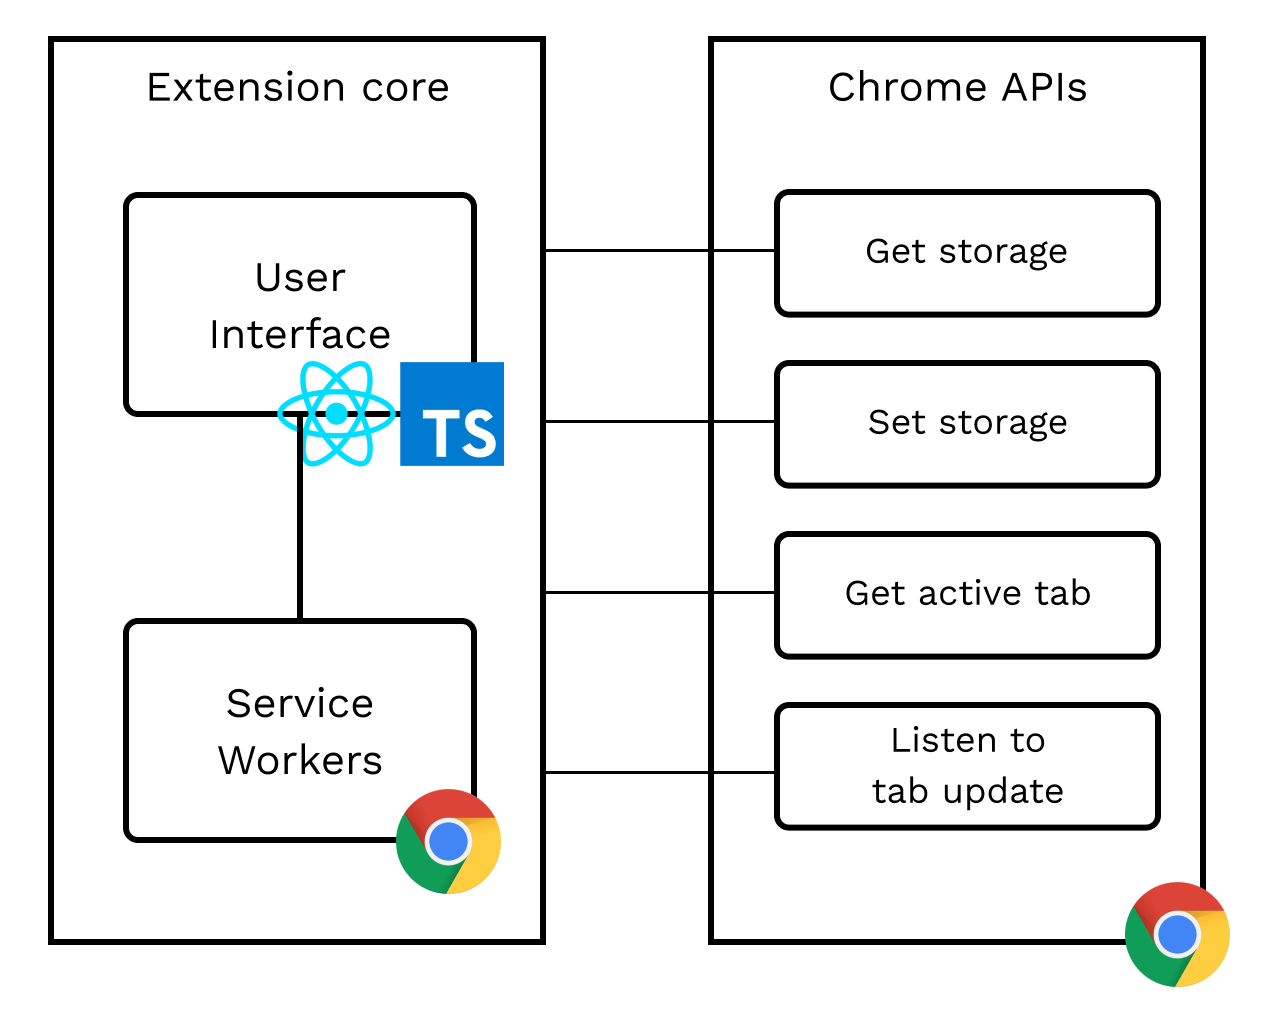
\includegraphics[width=0.7\textwidth]{assets/software_architecture_diagram.png}
  \caption{Software Architecture Diagram}
  \label{fig:softwareArchitectureDiagram}
\end{figure}


\section{Technologies}
\label{technologies_used}
Software architecture does more than just define the software's structure; it can also provide insight into what technologies may be required to build the software. The implementation browser decision will be presented in the next section. The implications of this change on various data storage mechanisms are discussed in the second section.

\subsection{Choice of Implementation Browser}
The selection of a browser was based on a number of factors. The first was the browser's usage rate. This is significant since anyone who doesn't already have the necessary browser will need to download and install it. Drop-outs due to the installation process or being unfamiliar with a new browser can significantly raise the cost of conducting the survey. The ease of use of the API and simplicity of implementation were additional crucial criteria. The extension programming process should ideally only need a basic understanding of the extension API. The capabilities of the API offered by the browser were another factor considered. The extension needs to:

\begin{enumerate}
  \item Store a big amount of data on the client side
  \item Read the URL - so the path and query string can be passed to the extension
  \item Modify the URL - so the most frequently used path and query string can be utilized
  \item Open a full-path URL in a new tab
  \item Access opened tabs
\end{enumerate}

\emph{Internet Explorer}\footnote{\emph{Internet Explorer} is a World Wide Web browser included with Microsoft Windows. Windows 10 deprecated the browser in favor of Microsoft's Edge Browser.} is officially retired and no longer supported as of June 15, 2022, after more than 25 years of facilitating web usage and experience. Consequently, Internet Explorer was removed from the list, leaving Firefox and Chromium-based browsers such as Google Chrome, Microsoft Edge, Opera, and Vivaldi as the only viable options.

Both the Firefox and Chrome extension APIs provide comparable functionality. Firefox's extension technology is, to a large extent, compatible with the extension API utilized by Chromium-based browsers. Most extensions designed for Chromium-based browsers operate in Firefox with very minor modifications. One disadvantage is that Mozilla only supports Manifest V2 and not V3. Since announcing Manifest V3 in 2018, Google has launched Manifest V3 in Chrome, started accepting Manifest V3 extensions in the Chrome Web Store, co-announced joining the W3C WebExtensions Community Group\footnote{The W3C WebExtensions Community Group is formed in collaboration with Apple, Microsoft, and Mozilla.} , and, most recently, laid out a timeline for Manifest V2 deprecation \autocite{alexei2021manifest}. Beginning in January 2022, no new Manifest V2 extensions will be accepted, and Manifest V2 will cease to function in January 2023. Manifest V3 mandates a change to the ecosystem that restricts Manifest V2 extensions and will likely require Manifest V2-based extensions to conform to Manifest V3 in the near future.

\begin{figure}[H]
  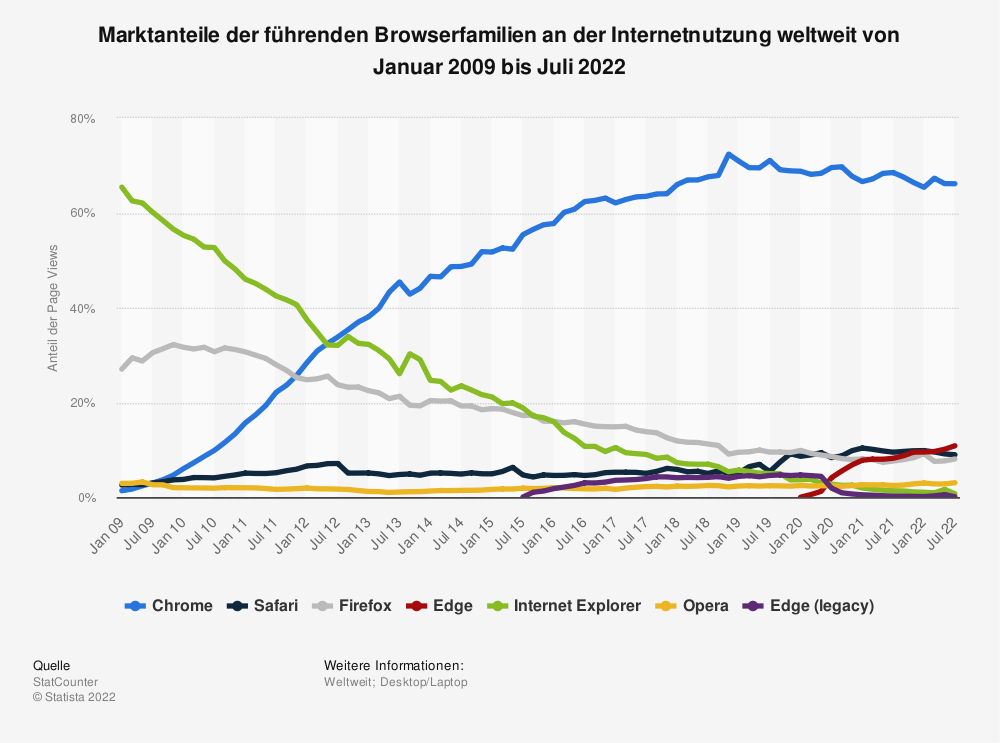
\includegraphics[width=\textwidth]{assets/statistic_id157944_marktanteile-fuehrender-browser-weltweit-bis-juli-2022.png}
  \caption{Market shares of leading browsers worldwide by July 2022}
  \label{fig:browserMarketShareChart}
\end{figure}

Additionally, it was discovered that the Chrome documentation was easy to grasp and was divided up into sections. Over two-thirds of all Internet users worldwide use Chrome as their primary browser (See \autoref{fig:browserMarketShareChart}). As a result, it was decided to develop a Chrome-based browser extension.

\subsection{Data storage}
Data can be stored either on the web server or the web client (the user's computer). Certain data types are better suited for one, while others perform more efficiently on the other. Sensitive and fragile data, for example, should always be stored on the server, whereas static data and user preferences can be stored on the client \autocite{macdonald2013html5}. Currently, most organizations manage various data aspects through various record systems. They have difficulty locating appropriate data stores because they report on each data source separately, resulting in complex data analytics processing. For this project, the types of data that must be stored are specified in \autoref{requirements_analysis}. Client-side storage is used to store and manipulate data in the browser, as no servers are required for this project. The following are instances of data storage and manipulation in the browser:

\begin{itemize}
  \item Maintaining the state of a client-side application, including the current screen, entered data, user preferences, etc.
  \item Utilities with strict privacy requirements that can access local data or files.
  \item Offline progressive web apps (PWAs)
\end{itemize}

\subsection*{Cookies}
HTTP cookies or Cookies were created to keep track of session data on the client side. According to the specification, a Set-Cookie HTTP header with session information was to be sent by the server as part of any response to an HTTP request. Here is an example of the headers in a server's response:

\begin{lstlisting}[language={}, caption={Cookie server response's headers}]
  HTTP/1.1 200 OK
  Content-type: text/html
  Set-Cookie: cookie=any
  Other-header: other-header-value
\end{lstlisting}

The cookie "cookie" with the value "any" is created by this HTTP response. The name and value are both URL-encoded before being sent. Session data is stored in the browser and retransmitted to the server with each request using the Cookie HTTP header, as shown in \autoref{lst:cookieHttpHeader}.

\begin{lstlisting}[language={}, caption={Cookie HTTP header}, label={lst:cookieHttpHeader}]
  GET /index.jsl HTTP/1.1
  Cookie: cookie=any
  Other-header: other-header-value
\end{lstlisting}

This additional data returned to the server can be used to determine the origin of the request. Although cookies provide a simple and well-supported storage mechanism, they have a number of drawbacks. To begin, each cookie is sent back and forth with each HTTP request (via HTTP headers), adding a significant amount of unnecessary overhead. Second, their storage capacity is far insufficient for modern web applications. Third, the same web application that uses cookies cannot run in multiple web browser tabs at the same time. Lastly, the API is somewhat cumbersome \autocite{kessin2011programming, macdonald2013html5}.

\subsection*{Web Storage}
Web storage was first addressed in the Web Applications 1.0 specification of the Web Hypertext Application Technical Working Group (WHAT-WG). Early development of this specification was incorporated into HTML5 before it was separated into its specification. Its purpose is to circumvent some of the limitations imposed by cookies when data is required only on the client side, without the need to constantly send data back to the server. The most recent revision of the Web Storage specification is the second edition. The Web Storage specification's two key goals are to provide a system for storing large amounts of data that survives between sessions and to provide a way to store session data outside of cookies \autocite{frisbie2019professional}.

The second edition of the Web Storage specification defines two types of storage: \texttt{localStorage}, for persistent data, and \texttt{sessionStorage}, for temporary data that is only kept for the duration of a single user session. Until the \texttt{localStorage} object is deleted either by JavaScript or the user by clearing the browser's cache, it will remain accessible. All information stored in \texttt{localStorage} will survive browser restarts, page refreshes, and the closing of all open windows and tabs. However, the \texttt{sessionStorage} object only stores information temporarily, until the browser is closed. This works in a similar way to a session cookie, except that it disappears when the browser is closed. Information saved to \texttt{sessionStorage} is preserved even after the page is refreshed, and depending on the browser's provider, may be accessible even if the browser crashes and is restarted. There are two different ways to store data in the browser that will persist through a page refresh, and both of these APIs are available in modern browsers. LocalStorage and SessionStorage are two types of window properties that have been widely supported by all major browser vendors since 2009.

There are restrictions with Web Storage, just like there are with other client-side data storage options. Some limitations can only be experienced in a certain browser. The client-side data size limit is typically determined per origin (protocol, domain, and port), giving each origin a predetermined amount of storage space. This prohibition is enforced by looking into where the storing page originated from. Aside from that, Web Storage uses synchronous operations, which will cause the main thread to become blocked. In addition, web workers and service workers are unable to access it, and the only type of data that it can store is strings.

\subsection*{IndexedDB}
The Indexed Database API, abbreviated IndexedDB, is a structured data store in the browser. IndexedDB was created as a replacement for the now-deprecated Web SQL Database API. The goal of IndexedDB was to create an API that allowed for the simple storage and retrieval of JavaScript objects while also allowing for querying and searching. IndexedDB is intended to be almost entirely asynchronous. As a result, the majority of operations are performed as requests that will be executed later and produce either a successful or an error result. To determine the outcome of nearly every IndexedDB operation, you must attach \texttt{onerror} and \texttt{onsuccess} event handlers.

It is a key-value browser-based NoSQL (Not Only SQL) data store that operates asynchronously. The NoSQL method of database management is an alternative to the more traditional relational and object-oriented schemas. Instead, NoSQL uses a key/value pair to store information. More than that, the database can store a lot of information, and its API allows for instant access to a practically infinite amount of organized data. But security was not a priority when designing IndexedDB, so it could be seen as insecure.

IndexedDB is a low-level API that necessitates extensive configuration before use, which can be a burden even when storing relatively straightforward information. Instead of relying on promises as most modern APIs do, it uses events instead. Wrappers for the IndexedDB library that provide promises, such as \emph{idb}\footnote{\emph{idb} is a small library that closely resembles the IndexedDB API, albeit with significant usability enhancements. GitHub repository: \url{https://github.com/jakearchibald/idb}}, hide both the powerful features and the complex machinery (such as transactions and schema versioning) that come with using the library.

\subsection*{Chrome Storage API}
Google Chrome provides an API called \texttt{chrome.storage}. This API has been optimized to meet the specific storage needs of extensions \autocite{chrome2021storage}. It allows you to directly synchronize data and persist data across tabs. Asynchronous storage ensures that scripts are not interrupted. As a result, asynchronous saving outperforms synchronous saving in terms of performance. The asynchronous behavior must be considered during implementation. Web Storage or \texttt{localStorage} has a maximum memory limit of 5 MB and does not support tab-spanning storage because the data is only available in the current context. The cross-tab storage and readout are required for the extension's development. Storage-wise, it's very similar to the \texttt{localStorage} API, but there are a few key distinctions:

\begin{itemize}
  \item User data can be synchronized in an automated fashion using \texttt{storage.sync}.
  \item Without requiring a background page, the content scripts of the extension can directly access user data.
  \item Even when using split incognito behavior, a user's extension settings can be saved.
  \item It is faster than the blocking and serial \texttt{localStorage} APIs because it is asynchronous with bulk read and write operations.
  \item Objects can be used to store user data\footnote{The \texttt{localStorage} API stores data in strings}.
  \item It is possible to read the administrator's enterprise policies for the extension using \texttt{storage.managed} with a schema.
\end{itemize}

Using \texttt{chrome.storage} can alleviate the aforementioned limitations with other client-side data storage solutions. Chrome Storage API is well-documented, simple, and takes very little time to set up. Data stored in \texttt{chrome.storage} can be accessed not only from tabs and windows of the same origin. As determined by the JSON stringification of each value and the length of each key, the maximum amount of data that can be stored in local storage is 5MB. However, this value can be ignored if \texttt{unlimitedStorage}\footnote{This permission is only applicable to Web SQL Database and application cache (See issue \url{https://bugs.chromium.org/p/chromium/issues/detail?id=58985}). Additionally, wildcard subdomains such as \url{http://*.example.com} are not supported at this time.} permission is used. Due to the limitations of HTML5 storage in the context of developing a Chrome Extension, the decision is made to use \texttt{chrome.storage}.

\newpage
\chapter{Project Implementation}

\newpage

\addcontentsline{toc}{section}{References}
\section*{References\markboth{References}{REFERENCES}}

\bibliographystyle{plain}
\bibliography{/Users/mba/Documents/htw/ba/ba-tex/thesis}

\newpage
\chapter{List of Abbreviations}

\begin{acronym}[WHAT-WG]
  \acro{API}{Application Program Interface}
  \acro{COM}{Component Object Model}
  \acro{CSS}{Cascading Style Sheets}
  \acro{DOM}{Document Object Model}
  \acro{HOC}{Higher-Order Components}
  \acro{HTML}{Hypertext Markup Language}
  \acro{HTTP}{Hypertext Transfer Protocol}
  \acro{HTTPS}{Hypertext Transfer Protocol Secure}
  \acro{IPC}{Inter-process Communication}
  \acro{JS}{JavaScript}
  \acro{JSON}{JavaScript Object Notation}
  \acro{JSX}{JavaScript XML}
  \acro{MB}{Megabyte}
  \acro{MVC}{Model-View-Controller}
  \acro{Props}{Properties}
  \acro{PWA}{Progressive Web Apps}
  \acro{UI}{User Interface}
  \acro{URI}{Uniform Resource Identifier}
  \acro{URL}{Uniform Resource Locator}
  \acro{UTM}{Urchin Tracking Module}
  \acro{WHAT-WG}{Web Hypertext Application Technical Working Group}
  \acro{XML}{Extensible Markup Language}
\end{acronym}

\newpage
\addcontentsline{toc}{section}{Eidesstattliche Erklärung}
%\section*{Eidesstattliche Erklärung}
\section*{Eidesstattliche Erklärung\markboth{EIDESSTATTLICHE ERKLÄRUNG}{EIDESSTATTLICHE ERKLÄRUNG}}

Ich erkläre hiermit an Eides Statt, dass ich die vorliegende Arbeit selbstständig und ohne Benutzung anderer als der angegebenen Hilfsmittel angefertigt habe; die aus fremden Quellen direkt oder indirekt übernommenen Gedanken sind als solche kenntlich gemacht. Die Arbeit wurde bisher in gleicher oder ähnlicher Form keiner anderen Prüfungskommission vorgelegt und auch nicht veröffentlicht.
\\
\\
Berlin, 22.08.2022
\\
\\
\\
\underline{\hspace{5cm}}
\\
Sunan Regi Maunakea


\end{document}  
